\documentclass[border=3pt,tikz]{standalone}
% Shared look for every TikZ figure in these notes.
% Included by each standalone figure file; also keeps the figures consistent
% with the colours used in the PDF and on the website.

\usepackage{tikz}
\usepackage{pgfplots}
\pgfplotsset{compat=1.18}
\usetikzlibrary{arrows.meta, decorations.markings, decorations.pathmorphing,
                patterns, calc, positioning}
\usepackage{amsmath}

% Series colours are the three validated categorical slots also used by the
% interactive widgets, so a path drawn in the printed notes and the same path on
% the website are the same colour. They clear the colour-vision-deficiency and
% contrast checks as a set; every path is direct-labelled as well, so colour is
% never the only thing carrying identity.
\definecolor{duPurple}{HTML}{68246D}
\definecolor{duBlue}{HTML}{2A78D6}
\definecolor{duRed}{HTML}{EB6834}
\definecolor{duGreen}{HTML}{1BAF7A}
\definecolor{duGrey}{HTML}{6B6B6B}

\tikzset{
  axisline/.style   = {-{Stealth[length=3mm]}, line width=0.7pt, black},
  path1/.style      = {duBlue,   line width=1.1pt},
  path2/.style      = {duRed,    line width=1.1pt},
  path3/.style      = {duGreen,  line width=1.1pt},
  statedot/.style   = {circle, fill=black, inner sep=1.4pt},
  arrowhead/.style  = {decoration={markings,
                        mark=at position #1 with {\arrow{Stealth[length=2.6mm]}}},
                       postaction={decorate}},
  lbl/.style        = {font=\small},
  slbl/.style       = {font=\footnotesize, duGrey},
  workfill/.style   = {duPurple, opacity=0.16},
}

\begin{document}
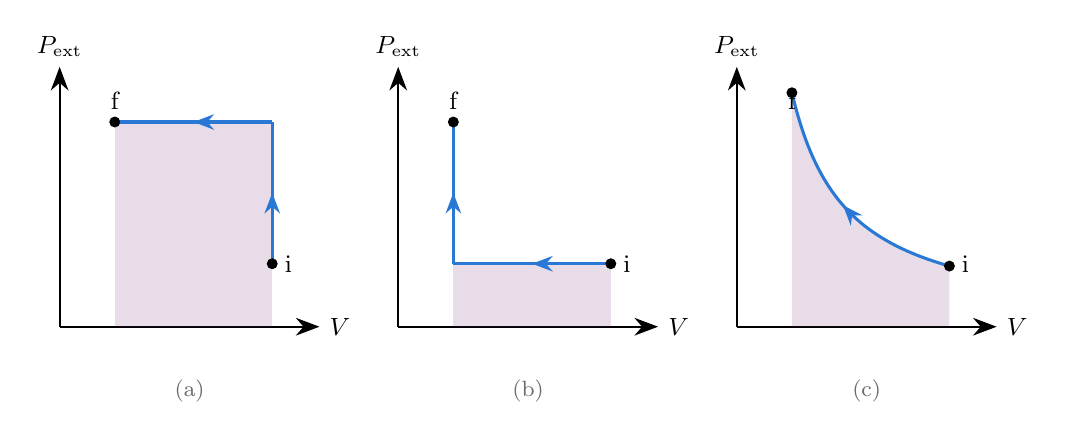
\begin{tikzpicture}[scale=1]

% ---- helper: one panel ----------------------------------------------------
\newcommand{\panel}[2]{%
  \begin{scope}[shift={(#1,0)}]
    \draw[axisline] (0,0) -- (3.3,0) node[right, lbl] {$V$};
    \draw[axisline] (0,0) -- (0,3.3) node[above, lbl] {$P_\text{ext}$};
    \node[slbl, below] at (1.65,-0.55) {(#2)};
  \end{scope}
}

% (a) compress at the HIGH pressure of state f: largest area
\panel{0}{a}
\begin{scope}[shift={(0,0)}]
  \fill[workfill] (0.7,0) rectangle (2.7,2.6);
  \draw[path1, arrowhead=0.5] (2.7,0.8) -- (2.7,2.6);
  \draw[path1, arrowhead=0.5] (2.7,2.6) -- (0.7,2.6);
  \node[statedot] at (2.7,0.8) {}; \node[lbl, right=1pt] at (2.7,0.8) {i};
  \node[statedot] at (0.7,2.6) {}; \node[lbl, above=1pt] at (0.7,2.6) {f};
\end{scope}

% (b) compress at the LOW pressure of state i: smallest area
\panel{4.3}{b}
\begin{scope}[shift={(4.3,0)}]
  \fill[workfill] (0.7,0) rectangle (2.7,0.8);
  \draw[path1, arrowhead=0.5] (2.7,0.8) -- (0.7,0.8);
  \draw[path1, arrowhead=0.5] (0.7,0.8) -- (0.7,2.6);
  \node[statedot] at (2.7,0.8) {}; \node[lbl, right=1pt] at (2.7,0.8) {i};
  \node[statedot] at (0.7,2.6) {}; \node[lbl, above=1pt] at (0.7,2.6) {f};
\end{scope}

% (c) quasi-equilibrium curve: in between
\panel{8.6}{c}
\begin{scope}[shift={(8.6,0)}]
  \fill[workfill]
    plot[domain=0.7:2.7, samples=60] (\x, {2.08/\x}) -- (2.7,0) -- (0.7,0) -- cycle;
  \draw[path1, arrowhead=0.5]
    plot[domain=2.7:0.7, samples=60] (\x, {2.08/\x});
  \node[statedot] at (2.7,{2.08/2.7}) {}; \node[lbl, right=1pt] at (2.7,0.8) {i};
  \node[statedot] at (0.7,{2.08/0.7}) {}; \node[lbl, above=1pt] at (0.7,2.6) {f};
\end{scope}

\end{tikzpicture}
\end{document}
